\documentclass[11pt]{ctexart}

\usepackage{geometry}
\geometry{a4paper, margin=2.5cm}
\usepackage{hyperref}
\usepackage{enumitem}
\usepackage{longtable}
\usepackage{array}
\usepackage{graphicx}

\title{Snooker2D 项目中期总结报告}
\author{井淳，鲁亦智，何广一 \quad 台球组}
\date{2026年7月14日}

\begin{document}

\maketitle

\section{项目概况}

Snooker2D 是一个基于 C++17 和 Qt 6 的 2D 斯诺克台球游戏，采用课程讲授的 MVVM 五层架构。项目三人协作，10 天工期，当前处于中期检查节点。

\section{技术架构}

\subsection{分层设计}

项目拆分为四层编译目标，App 层在主可执行文件中完成装配：

\begin{center}
\begin{tabular}{|c|l|l|}
\hline
\textbf{层} & \textbf{职责} & \textbf{编译依赖} \\
\hline
Common & 全局类型、常量、工具函数、DTO & 无 \\
Model & 游戏状态机、物理引擎、规则判定 & Common + Qt::Core \\
ViewModel & 数据翻译、状态推送、命令处理 & Model + Common + Qt::Core \\
View & 界面渲染、用户输入 & Common + Qt::Widgets \\
App & 对象装配、信号槽绑定 & 所有层 \\
\hline
\end{tabular}
\end{center}

关键约束：View 层不链接 ViewModel/Model（CMake 编译期强制）。

\subsection{层间通信}

ViewModel 和 View 的跨层信号槽由 App 层在 App.cpp 中集中绑定（10 条 connect）。Model 到 ViewModel 的通知绑定在 ViewModel 构造函数内部完成。

\begin{center}
\begin{tabular}{|c|c|c|c|}
\hline
\textbf{绑定类型} & \textbf{方向} & \textbf{连接位置} & \textbf{数量} \\
\hline
属性绑定 & ViewModel → View & App.cpp & 5 \\
命令绑定 & View → ViewModel & App.cpp & 5 \\
通知绑定 & Model → ViewModel & ViewModel 构造 & 9 \\
\hline
\end{tabular}
\end{center}

\section{已完成功能}

\begin{itemize}
\item 斯诺克标准 22 颗球的初始摆球和球桌渲染
\item 鼠标瞄准与击球（含球杆动画）
\item 力度/角度双模控制（滑块 + 鼠标拖动）
\item 球-球弹性碰撞、球-库边反弹、摩擦力减速
\item 袋口检测与落袋、D 区白球复位
\item 计分板、游戏信息面板、比赛重启
\item 60 条 Common 层单元测试、架构护栏自动检查
\end{itemize}

\section{分工完成情况}

\subsection{鲁亦智（开发者 A）— View 层}

负责球桌渲染、鼠标交互、球杆动画、控件布局，共实现 GameView、CueControl、ScoreBoard、GameInfoPanel、MainWindow 五个 View 组件。所有 View 组件仅依赖 Common 层的 ViewState DTO 和 Qt::Widgets，编译期不链接 ViewModel/Model。

\textbf{GameView（球桌视图）}：paintEvent 中实现六步绘制管线——深灰背景填充、绿色台面与棕色库边、D 区白球放置引导（半透明弧线区域+竖线）、6 个黑色袋口、22 颗球（按 BallType 着色，白球/黑球特殊描边色，每球左上角 35\% 大小白色高光模拟 3D 效果）、瞄准辅助虚线、球杆动画。resizeEvent 中根据窗口宽高比自动适配 2:1 比例的球桌矩形，保证球桌始终占视图 90\% 且不变形。gameToPixel/pixelToGame 双向坐标转换方法通过 centeredCoordinates 标志自动切换居中坐标系（物理引擎使用）和左上角坐标系（球桌坐标）。

\textbf{球杆动画与鼠标交互}：将击球操作从按钮改为全鼠标操作——setMouseTracking(true) 开启鼠标追踪，mouseMoveEvent 中通过 atan2 实时计算鼠标相对于白球的方位角并 emit angleChanged；wheelEvent 以每格 5\% 步进调节击球力度并 emit powerChanged；mousePressEvent 中按下左键触发 playShotAnimation，启动 16ms 定时器，每帧将球杆间隙递减 10 像素直到归零，动画结束时 hideAimingTools 隐藏瞄准工具并 emit shotAnimationFinished 通知 ViewModel 进入物理模拟。drawCue 中使用 QLinearGradient 实现球杆木纹渐变效果（深棕→浅棕→米黄），杆头单独着色。

\textbf{辅助控件}：CueControl 实现双滑块面板——角度滑块（0-359°）和力度滑块（0-100\%），applyCueState 槽中使用 blockSignals 避免滑块反馈环路。ScoreBoard 展示双方总分、单杆得分、犯规信息和比赛状态，大字体得分突出显示。GameInfoPanel 通过 phaseStyleSheet 方法根据 GamePhase 枚举（红球/彩球/犯规/自由球/结束）为阶段标签应用不同颜色样式，D 区放置提示仅在 showWhiteBallPlacementHint 为真时显示。MainWindow 作为纯布局容器，setupUI 中以 3:1 比例左右分栏——左侧放置 GameView + CueControl（上下排列），右侧放置 ScoreBoard + GameInfoPanel，通过 4 个 getter 暴露子 View 供 App 层绑定信号槽。

\textbf{技术难点}：坐标系转换——物理引擎使用以球桌中心为原点的居中坐标系，而 QPainter 绘制需要左上角像素坐标，通过 centeredCoordinates 标志在 gameToPixel/pixelToGame 中自动偏移 TABLE\_WIDTH/2 和 TABLE\_HEIGHT/2 解决。球杆动画与鼠标事件的时序配合——动画期间（m\_isShotAnimating 为真）需要阻止鼠标交互（updateCueAngleFromMouse 和 wheelEvent 均检查 aimingToolsVisible），动画结束后通过 hideAimingTools 标志等待 ViewModel 的 applyTableState 更新 canAim 才恢复显示瞄准工具，避免击球动画与下一次瞄准的视觉重叠。

\subsection{何广一（开发者 B）— Model + ViewModel 层}

负责游戏状态机、物理引擎、规则判定、数据翻译和状态推送。

\textbf{物理引擎}：固定时间步长（1/60s）的六步模拟流程——运动、球-球碰撞、球-库边碰撞、袋口检测、摩擦减速、硬边界约束。球-球碰撞采用等质量弹性碰撞公式，库边碰撞通过 closestPointOnSegment 计算接触点法线。

\textbf{规则引擎}：FoulResult 结构体承载犯规类型、描述文本和罚分。checkFoul 按优先级检测白球落袋、空杆、先击错球、无球碰库四种犯规。

\textbf{GameSessionViewModel}：唯一的 ViewModel 协调器。构造时连接 Model 的 9 个信号到内部处理槽。5 个 pushXxxState() 方法从 Model 读取数据、构造 ViewState DTO、emit 到 View。5 个 public slots 接收 View 命令。

\textbf{技术难点}：物理参数的经验性调优（恢复系数 0.96→0.88、库边弹性 0.77 的多轮试错）、库边碰撞中 closestPointOnSegment 的应用。

\subsection{井淳（开发者 C）— Common + App 层}

负责公共类型与工具、ViewState DTO 设计、跨层信号槽装配、构建配置和项目管理。

\subsubsection{Common 层设计}

Common 层的设计目标是提供所有层共用的基础定义，使上层代码能脱离具体实现进行编译。分为两类：核心子层（纯 C++，不依赖 Qt）定义全局类型、物理常量和数学工具函数；DTO 子层定义 View 和 ViewModel 之间的数据交换格式（ViewState 结构体）。关键设计决策包括：FoulResult 结构体放在 Model 层而非 Common 层（因其含 QString 成员依赖 Qt）；袋口坐标由 Model 层 Table 类管理而非散落在常量文件中；Vector2D 的 14 个运算符中成员函数委托给自由函数实现，避免代码重复。

\subsubsection{App 层设计}

App 层的设计目标是将 MVVM 各层的信号槽集中装配，使 View 和 ViewModel 可以独立开发、各自声明自己的信号与槽，互不感知对方的存在。App::run() 是唯一的装配入口——创建 GameSessionViewModel 实例、通过 MainWindow 的 getter 获取 4 个 View 子控件、随后以 10 条 QObject::connect 完成全部跨层绑定。其中属性绑定 5 条（ViewModel 的 tableStateReady 等信号连接到 View 的 applyXxxState 槽），命令绑定 5 条（View 的 angleChanged 等信号连接到 ViewModel 的 setAngle 等槽）。通知绑定（Model 信号到 ViewModel 槽）保留在 GameSessionViewModel 构造函数内部，因为 ViewModel 本就持有 Model 指针并直接调用其方法，两者是翻译关系而非解耦关系。

该方案经历了三轮架构迭代才收敛到当前形态。最初使用 GameUiBus 作为通信中间件，View 和 ViewModel 通过 Bus 信号间接通信。随后发现 Bus 在新增信号时会导致所有依赖 Common 层的 View 重编译，且 Bus 自身不属于任何一层——违背了 MVVM 的边界约束。第二轮删除了 3 个子 ViewModel 并合并到 GameSessionViewModel，减少了 ViewModel 内部转发。第三轮完全取消 Bus，各层自管 signal/slot 声明，App 层集中 connect。当前方案中 View 只依赖 Common 层（GameViewState.h），ViewModel 不依赖 View，编译依赖由 CMake 强制执行。

\subsubsection{构建配置与测试}

CMake 将项目编译为四层 target（common / model / viewmodel / view），其中 View 层的 CMake 配置不链接 ViewModel 和 Model，从编译层面杜绝了架构违规。架构护栏脚本作为 CMake custom target 持续验证 MVVM 边界。Common 层 60 条单元测试覆盖全部向量运算、几何函数、运算符和类型辅助函数，无第三方测试框架依赖。

\section{团队协作}

三位成员通过 Git 协作，提交遵循 \texttt{type(layer): description} 规范。

\textbf{提交统计}：

\begin{center}
\begin{tabular}{|c|c|c|}
\hline
\textbf{姓名} & \textbf{提交数} & \textbf{负责层} \\
\hline
鲁亦智（A） & 14 & View \\
何广一（B） & 8 & Model / ViewModel \\
井淳（C） & 13 & Common / App / 文档 \\
\hline
\end{tabular}
\end{center}

MVVM 分层让三个人能真正并行推进——View 在 Model 还没写完的时候就能用 DTO 骨架做界面，各层之间的接口通过 Git 历史能追踪到，中间没出过编译失败级别的对接问题。下面是我们目前的 commit 记录：

\begin{center}
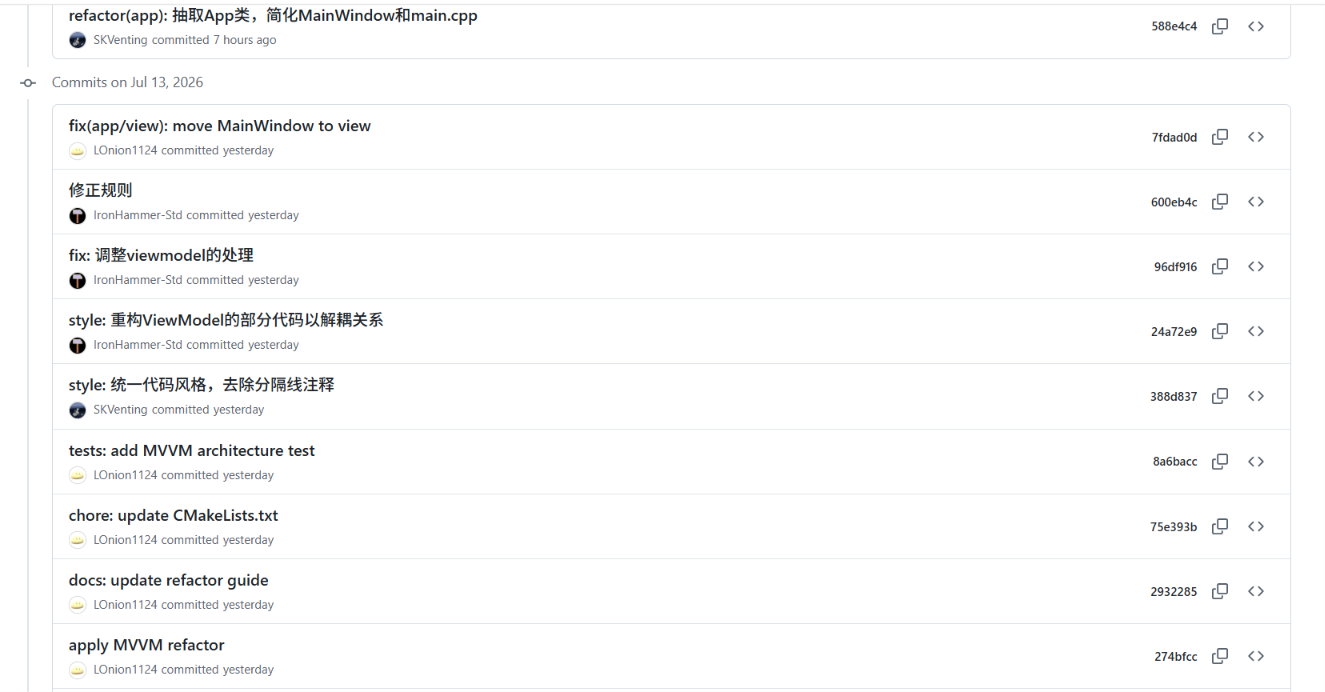
\includegraphics[width=0.9\textwidth]{imgs/commit_hist.png}
\end{center}

项目经历了好几次架构调整，从引入 GameUiBus 到删除子 ViewModel，再到现在的 App 集中绑定。每次改架构都是三个人一起讨论完再动手，中间也走过弯路，但慢慢才收敛到现在这个比较干净的结构。

\section{阶段性成果展示}

\begin{center}

\includegraphics[width=0.85\textwidth]{imgs/main_window.png}
\\[0.3cm]
{\small 游戏主窗口}

\vspace{1.0cm}

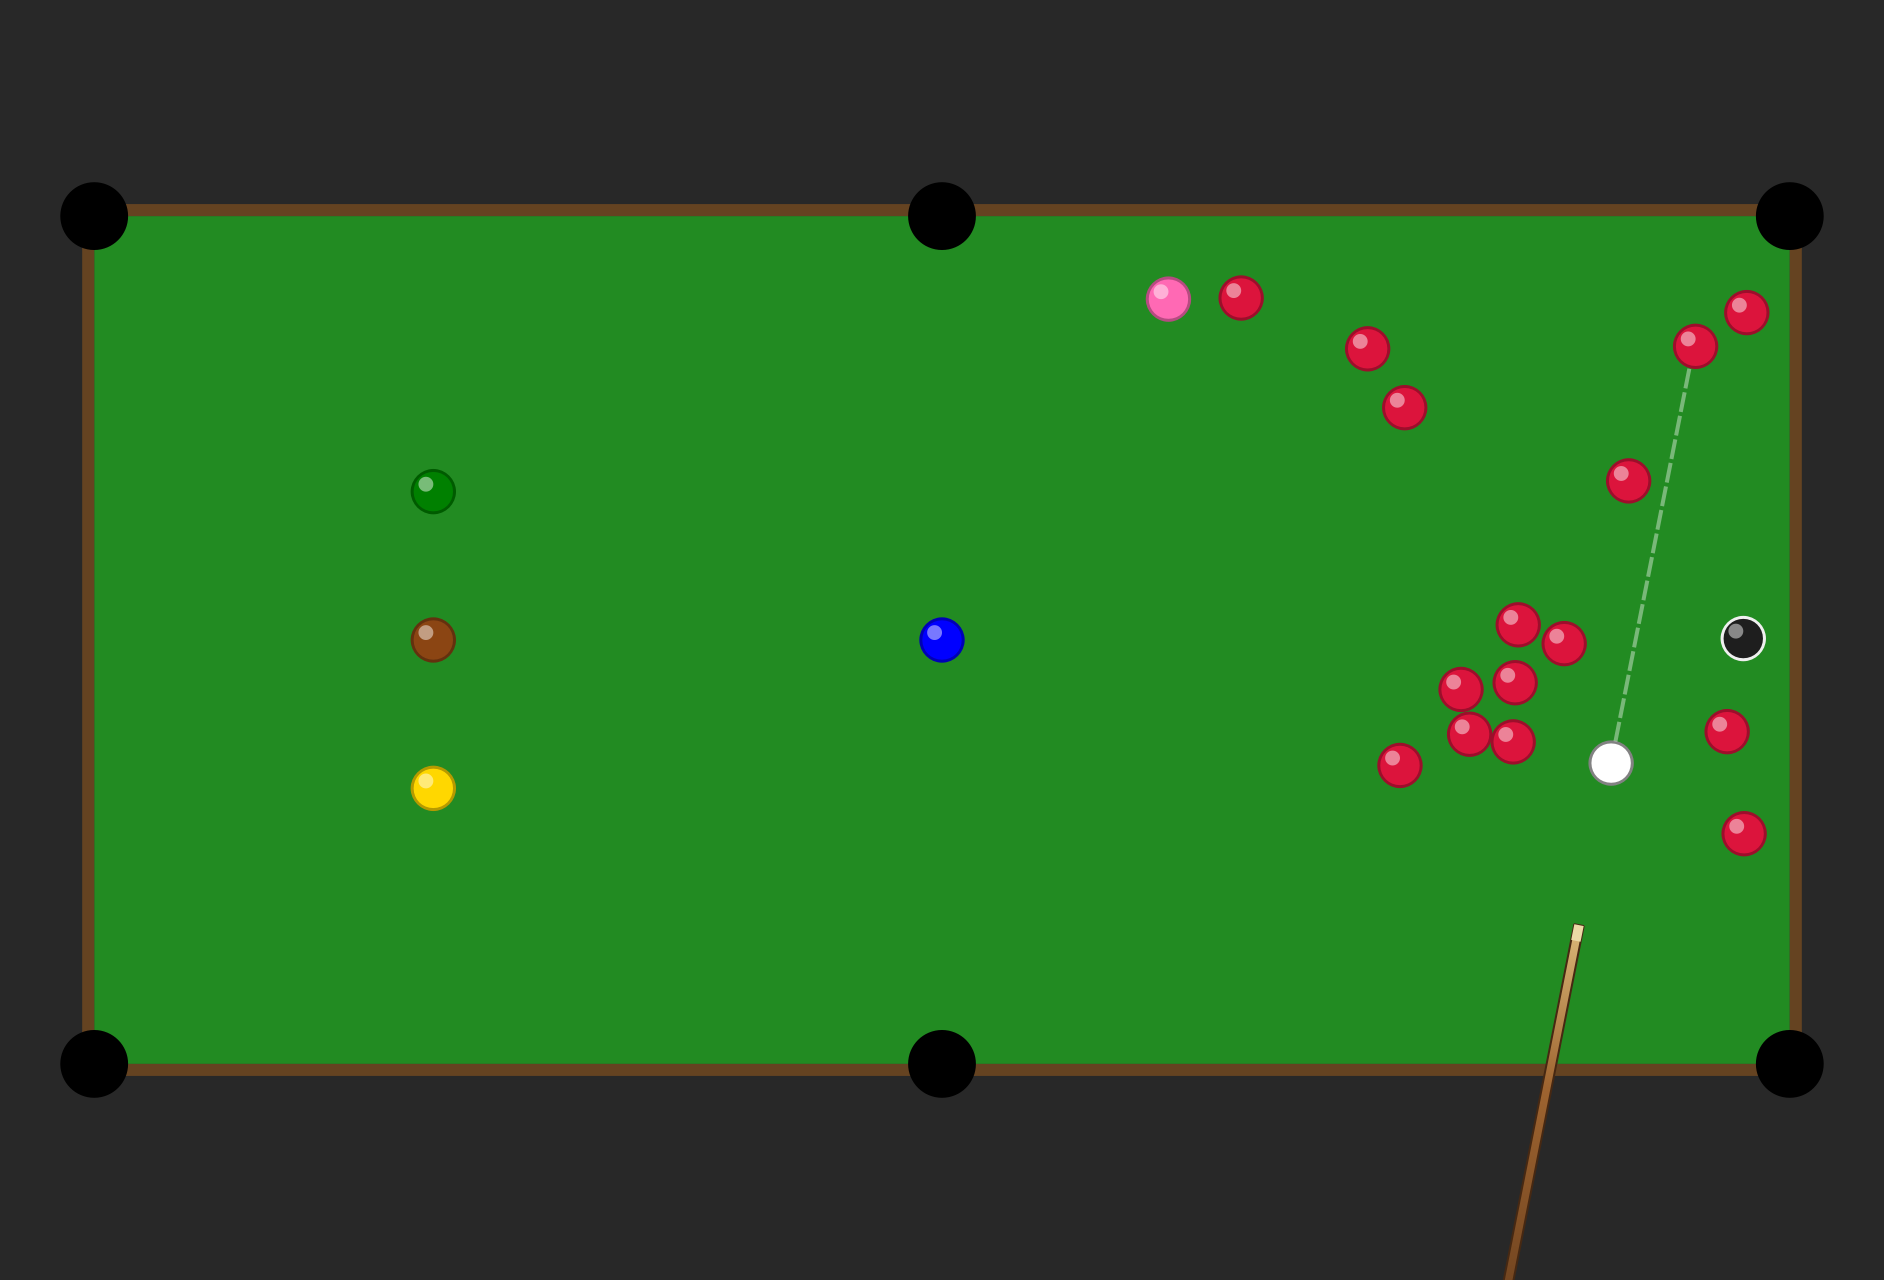
\includegraphics[width=0.85\textwidth]{imgs/hit_ball.png}
\\[0.3cm]
{\small 物理碰撞效果}

\vspace{1.0cm}


\includegraphics[width=0.85\textwidth]{imgs/place_ball.png}
\\[0.3cm]
{\small D 区白球复位}
\end{center}

\section{个人反思与收获}

\subsection{鲁亦智}

View 层开发让我深刻体会到 MVVM 架构中"数据驱动界面"的含义——所有绘制都来自 ViewModel 的属性变更通知，View 自身不主动管理刷新时机。applyTableState 是唯一的更新入口，缓存 ViewState 后调用 update() 触发 Qt 重绘。这种单向数据流使得 View 层的调试变得简单：只要检查 applyTableState 收到的 DTO 内容是否正确，就能定位问题是在 ViewModel 的数据转换还是 View 的渲染逻辑。DTO 中 canAim/canShoot/isPlacingWhiteBall/isSimulating 等布尔字段的设计也让 View 无需引入任何游戏规则知识——例如 aimingToolsVisible() 方法仅通过组合这些布尔值判断是否显示瞄准工具，完全不需要理解"什么情况下可以瞄准"的游戏语义。

鼠标交互的实现比预期复杂得多。从最初的按钮触发击球到全鼠标操作，经历了角度计算（atan2 坐标系转换，角度归一化到 0-360°）、坐标变换（像素坐标→游戏坐标→球桌坐标的三级映射）、动画衔接（16ms 定时器驱动球杆间隙逐帧递减，需精确控制动画期间的事件屏蔽与结束后的状态恢复）、事件过滤（放置白球模式、动画播放中、模拟运行中三种场景下需分别处理鼠标事件的优先级）等多个细节的处理。特别是 aimingToolsVisible 方法的设计——需要同时考虑 isPlacingWhiteBall（放置模式不显示瞄准）、hideAimingTools（击球后隐藏直到下一轮）、m\_isShotAnimating（动画期间仅显示球杆）三种状态的组合——这个看似简单的布尔判断实际上经历了多次 bug 修复才稳定。

与 C 的协作中，App 层的信号连接经历了按钮击球→鼠标击球→GameUiBus 中间件→直接绑定的多次重构。每次架构变迁都意味着 View 暴露的信号签名需要重新协商——例如从 clicked() 改为 angleChanged(double)/powerChanged(double)/shotAnimationFinished()，再到 whiteBallPlacementRequested(double, double) 的加入。MainWindow 从最初包含信号连接逻辑到最终退化为纯布局容器+getter 暴露，体现了"装配逻辑集中到 App 层"这一原则的逐步明晰。与 B 的跨层协作中，最大的收获是"约定优于实现"——只要 ViewState DTO 的字段语义和信号签名在 Common 层约定清楚，View 和 ViewModel 可以真正并行开发：我在 GameView 中开发球杆动画时，B 甚至还没有完成物理引擎的击球回调，但因为我只需要 emit shotAnimationFinished() 信号，双方的工作完全解耦。

\subsection{何广一}

Model 层开发最核心的挑战不在于物理公式本身，而在于处理“不完美的现实”——球碰撞恢复系数、库边不同弹性、摩擦力非线性，这些细节在理论推导中被简化，但在视觉反馈中会暴露。多次参数试错让我理解了物理引擎调优需要耐心。ViewModel 层的设计让我体会到接口设计的权衡：暴露太少 View 无法工作，暴露太多则性能和维护成本上升。与 A 和 C 的跨层协作中，最大的收获是“约定优于实现”——只要层间信号签名约定清楚，三方可以真正并行。

\subsection{井淳}

作为 Common 层和 App 层的负责人，我承担了“基础设施提供者”和“装配工人”的双重角色。Common 层要求对需求的预判——Vector2D 的复合赋值运算符在一开始看似多余，但当物理引擎要求就地更新速度向量时立刻体现价值。App 层要求对所有层接口的全局理解——每一条 connect 都意味着理解一个信号的来源和去向。

与 B 的协作让我认识到，分层架构中的灰色地带需要灵活处理——B 在物理调优时修改了 Common 层文件，严格来说超出了分工约定，但为了迭代效率我选择了接受而非回退。三轮架构重构（Bus 引入→子 VM 合并→Bus 取消）让我切身体会了架构设计的权衡——没有一劳永逸的方案，只有在实践中持续迭代的改进。

\section{智能体的使用}

本项目选择以人为主的开发模式。大模型智能体在开发中仅用于补充性工作：代码补全与格式化、文档草稿生成、构建配置调试建议。所有核心架构设计、接口协调、技术决策均由团队成员自主完成。

\section{后续计划}

\begin{enumerate}[leftmargin=*]
\item 完善斯诺克规则引擎（犯规判定全部场景、自由球、输赢判定）
\item 补充 Model 层单元测试和端到端集成测试
\item CI/CD 配置
\item UI 美化与资源整理
\item 文档完善
\end{enumerate}

\end{document}
